\documentclass[12pt]{article}
\usepackage{fix-cm}

\usepackage[a4paper,
            top=3cm, bottom=2cm,
            left=3cm, right=2cm]{geometry}

\usepackage[num, overcite]{abntex2cite}
\citebrackets[]
\makeatletter
\renewcommand\@biblabel[1]{[#1] }
\makeatother

\usepackage{subcaption}
\usepackage{booktabs}
\usepackage{amsmath, amsfonts, amsthm, bm}
\usepackage{newtxtext, newtxmath, mathtools}
\usepackage[brazil]{babel}
\usepackage[T1]{fontenc}
\usepackage{indentfirst}
\usepackage{microtype}
\usepackage{fancyhdr}
\usepackage{graphicx}
\usepackage{ragged2e}
\usepackage{multirow}
\usepackage{setspace}
\usepackage{subfig}
\usepackage{icomma}
\usepackage{array}
\usepackage{float}
\usepackage{tikz}

\usepackage{silence}
\WarningFilter{latex}{Command \showhyphens has changed}

\onehalfspacing
\setlength{\parindent}{1.25cm}
\setlength{\parskip}{0.4\baselineskip}
\justifying

\usepackage{titlesec}

\newcommand{\titlefix}{
  \hyphenpenalty=10000
  \exhyphenpenalty=10000
  \emergencystretch=2em
}

\captionsetup{
    justification=centering
}

\titleformat{\section}
{\normalsize\bfseries\titlefix}
{\thesection.}
{0.5em}
{}

\titlespacing*{\section}
{0.75cm}
{1.5\baselineskip}
{0.8\baselineskip}

\titleformat{\subsection}
{\normalsize\bfseries\titlefix}
{\thesubsection.}
{0.5em}
{}

\titlespacing*{\subsection}
{1.5cm}
{1.2\baselineskip}
{0.6\baselineskip}

\titleformat{\subsubsection}
{\normalsize\bfseries\titlefix}
{\thesubsubsection.}
{0.5em}
{}

\titlespacing*{\subsubsection}
{2.25cm}
{1.0\baselineskip}
{0.4\baselineskip}

\titleformat{name=\section,numberless}
{\normalsize\bfseries\centering\titlefix}
{}
{0em}
{}

\titlespacing*{name=\section,numberless}
{0cm}
{1.5\baselineskip}
{0.8\baselineskip}

\begin{document}
\pagestyle{empty}

\begin{center}

	
\includegraphics[width=0.3\textwidth]{ita_rgb.jpg}

	\vfill

	{\large\bfseries
		Relatório parcial semana 1\\[2.0\baselineskip]

	}

	\vfill

	{\normalsize\bfseries
		Caio Schaden Ishida\\[0.5\baselineskip]
		Cauã Henrique de Souza\\[0.5\baselineskip]
		Felipe Osternes da Silva\\[0.5\baselineskip]
		Henrique Sousa Fagundes\\[0.5\baselineskip]
		João Victor Evers Cordeiro\\[0.5\baselineskip]
		José Hernando Figueiredo da Silva Filho
	}

	\vfill

	{\normalsize\bfseries
		Grupo nº 07\\[0.6\baselineskip]
		Turma 30.2
	}

	\vfill

	{\normalsize
		Professores\\
		Deborah Dibbern Brunelli\\
		Leonardo Tsuyoshi Ueno\\
		Luís Gustavo Ferroni Pereira\\

		\medskip
		
		Data de entrega: 11/08/2026
	}

	\vfill

	{\normalsize\bfseries
		Departamento de Química\\
		Divisão de Ciências Fundamentais\\
		Instituto Tecnológico de Aeronáutica - ITA
	}

\end{center}

\newpage

\section{Atividades da semana 1}
Durante a semana 1, foi criado um repositório no \textit{github}\cite{ishida_doe} (\textit{software} de desenvolvimento colaborativo) para organizar a árvore de arquivos gerada no desenvolvimento da aplicação. Também, foi implementado o primeiro protótipo em MATLAB do ajuste por mínimos quadrados\cite{barrosneto2001} para um modelo quadrático de duas variáveis. A partir do ajuste, é possível determinar o valor máximo e o ponto no qual ele ocorre.

Ao executar o arquivo ``.m'', o programa gera uma sequência de caixas de diálogo, assim como mostra na Figura \ref{fig:dialogboxes}, nas quais o usuário é instruído a fornecer os nomes e as unidades das variávies e do valor a ser maximizado, e os limites da região experimental. Em seguida, são fornecidos ao usuário os nove pontos da região experimental, conforme um planejamento composto central com $\alpha = 1$ sem duplicatas, nos quais devem ser realizados ensaios cujos resultados são então fornecidos em novas caixas de diálogo. Por fim, o valor e o ponto de máximo dentro da região experimental são retornados ao usuário. A Figura \ref{fig:dialogboxes} mostra, na ordem que são exibidas ao usuário, as caixas de diálogo, omitindo a entrada dos resultados para os ensaios 1 a 9.

\begin{figure}[H]
	\centering
	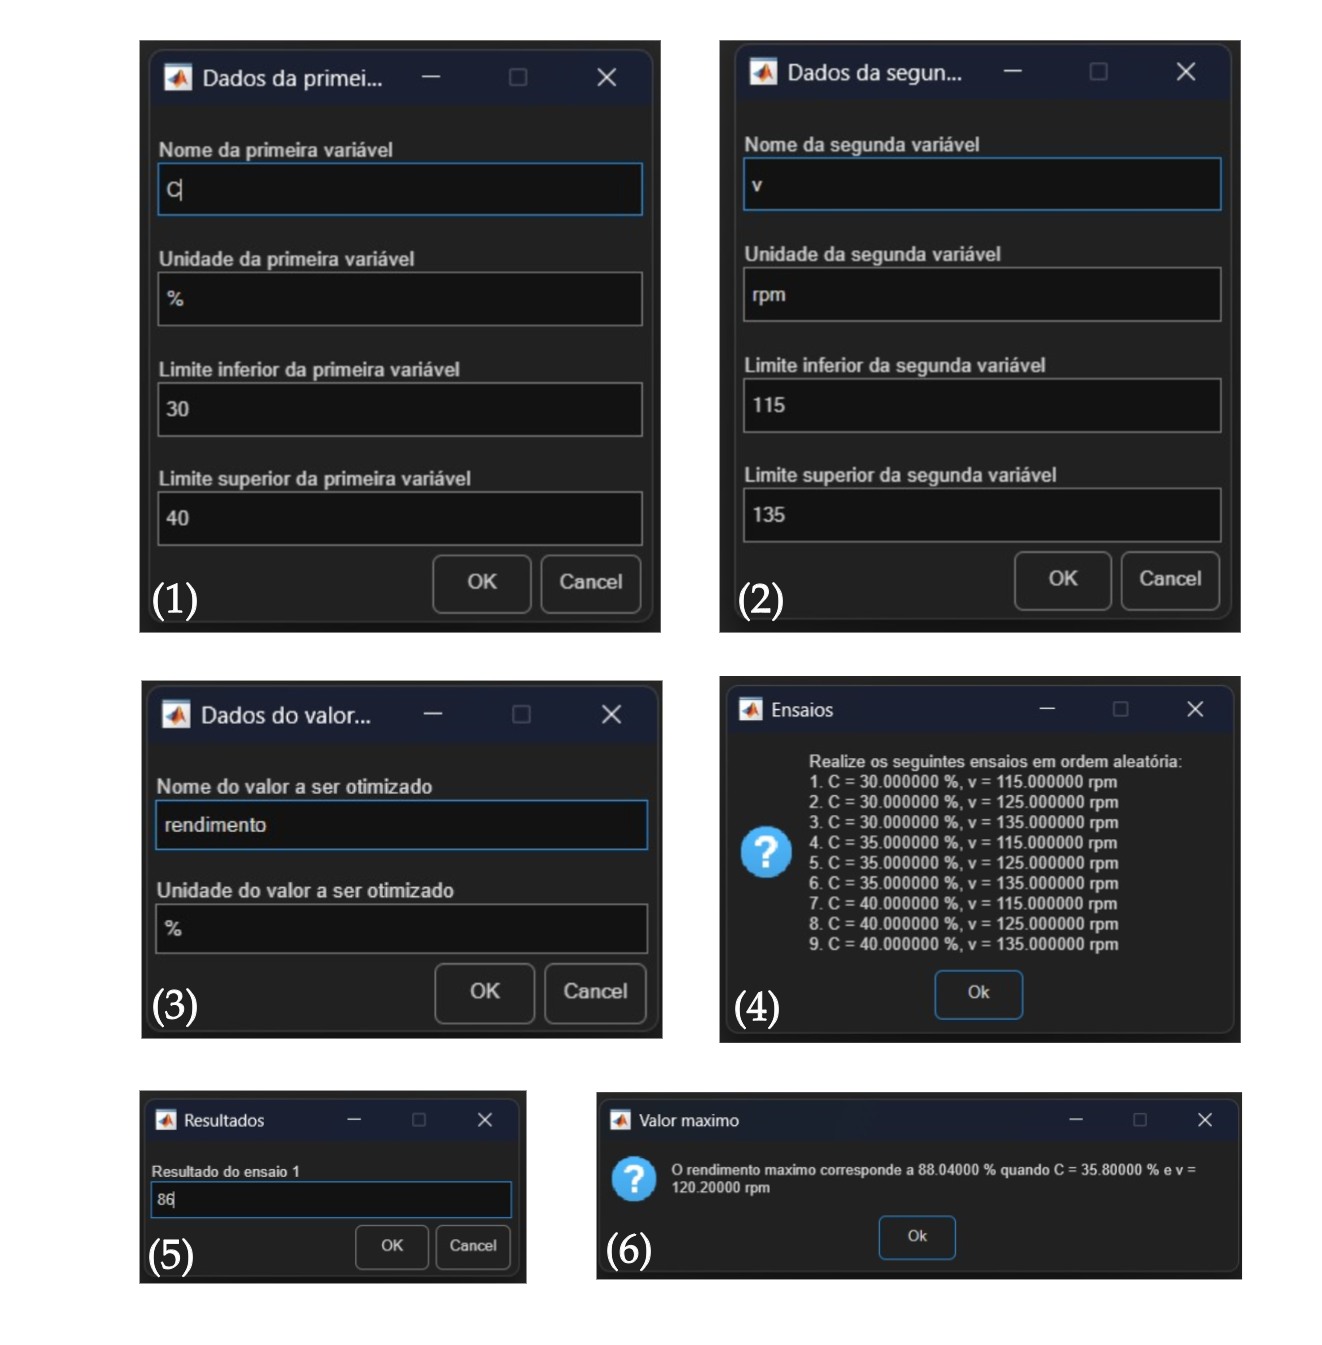
\includegraphics[width = 0.8\linewidth]{dialogboxes.png}
	\caption{Sequência de caixas de diálogo ao executar a aplicação}
	\label{fig:dialogboxes}
\end{figure}

\section{Planejamento para a semana 2}
O principal objetivo para a semana 2 é continuar e aperfeiçoar o trabalho de prototipagem desenvolvido na semana 1. Dentre as principais metas, as prioridades serão adaptar o programa para funcionar com 3 variáveis e realizar uma exploração mais precisa da região experimental com outros valores de $\alpha$ e com a realização de duplicatas em torno do ponto central do planejamento. Ainda, pretende-se implementar um algoritmo de análise de dados por meio do qual a aplicação forneça automaticamente a tabela de Análise de Variância (ANOVA) em diferentes formatos, como \textit{latex} ou ``.png'', e o gráfico adequado dos resultados experimentais, que pode ser ternário, 3D, em curvas de nível \textit{etc}. Por fim, pretende-se aperfeiçoar a interface e configurabilidade do aplicativo, adicionando a opção de performar apenas a análise de dados ou o planejamento experimental e simplificando a interface de entrada para os resultados dos ensaios por meio de uma planilha.

A Tabela \ref{tab:taskmng} é a atribuição de tarefas para cada um dos integrantes do grupo para a próxima semana. 

\begin{table}[H]
    \centering
    \caption{Atribuição de tarefas para a semana 2}
    \begin{tabular}{l p{10cm}} 
        \toprule
        \textbf{Integrante} & \textbf{Atividade} \\
        \midrule  
        Caio Schaden & Revisar as demais atividades \\
        Cauã Souza & Implementar a entrada dos resultados de ensaios experimentais por meio de uma planilha \\
        Henrique Fagundes & Estudar a compilação do \textit{software} e a interface interativa \\
        Felipe Osternes & Implementar sistema que identifique em qual etapa da experimentação o grupo que utiliza o aplicativo está \\
        José Hernando & Extensão da aplicação para aceitar três fatores e documentação do código \\
        João Evers & Implementar a análise de dados com o gráfico e a tabela de ANOVA \\
        \bottomrule
    \end{tabular}
    \label{tab:taskmng}
\end{table}

\newpage

\section*{Referências bibliográficas}
\begingroup
\renewcommand{\section}[2]{}
\bibliography{referencias}
\endgroup

\end{document}
